\section{Recurrent Neural Networks \label{ssec: RNNs}}
    Consider the following sentences as inputs to a NN: 
    
    \begin{table}[h]
    \begin{tabular}{|l|l|l|l|l|l|}
        \hline
        $i$   & 0   & 1   & 2     & 3    & 4    \\ \hline
        $s_1$ & The & sky & isn't & blue &      \\ \hline
        $s_2$ & The & sky & is    & blue &      \\ \hline
        $s_3$ & The & sky & is    & not  & blue \\ \hline
    \end{tabular}
    \centering
    \end{table}
    
    Using word embeddings (see Sec. \ref{ssec: word embeddings}) we are able to turn these words into numbers that the NN can process, but due to the (lack of) structure within sentences, we face another issue:
    Sentences $s_1$ and $s_2$ have different meanings, but because most words are the same, the inputs would appear relatively similar to the model and yield similar outputs $\hat{Y}$. $s_1$ and $s_3$ have the same meaning, but are of different length. In our hypothetical NN, the inputs in positions $i = \{2, 3, 4\}$ are different, leading to potentially quite different outputs $\hat{Y}$.
    
    The problem is that in language, the absolute position of words within sentences is not particularly important, but context is extremely important: One word, "not", can change the meaning of the entire sentence dramatically.
    
    \begin{figure}[h]
        \centering
        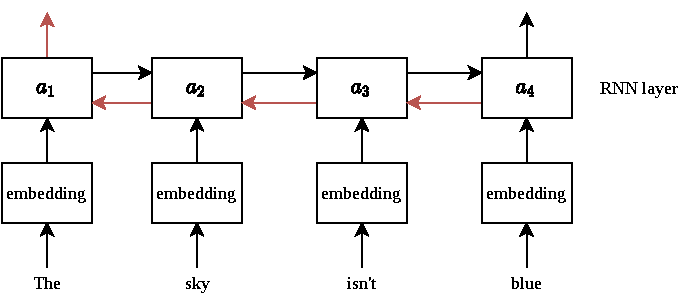
\includegraphics{rnn.pdf}
        \caption{The RNN layer is given an input sequence of word embeddings, calculates a hidden state depending on the first embedding and the weights of the first neuron, and passes this hidden state on to the next neuron within the RNN layer. Every neuron modifies the hidden state based on its weights and the input embedding at its position and passes the modified state on. At the end of the sentence, the hidden state is passed on as the output of the layer. In a bidirectional model (red arrows), a second hidden state is passed through the layer ``backwards".}
        \label{fig:rnn}
    \end{figure}
    
    Recurrent neural networks (RNNs) address these concerns and can process sequences of variable length such as sentences. RNNs use neurons as computational units in the same way traditional NNs do, but instead of simply connecting neurons from the previous layer to neurons of the next layer, they connect neurons within a single layer, so that they form a directed graph. Every neuron $n_i$ then corresponds to one entry in the sequence (e.g. one word in a sentence) and calculations are performed in a temporal direction: a hidden state of numbers is created at $n_0$, and repeatedly passed on to the next node $n_{i+1}$, changed in a way determined by the $i+1$th entry and the neuron's parameters $\theta$ and passed on again. At the last neuron, every entry has impacted the hidden state in some sensible way and the information can be passed to the next layer for further processing. A short example is given in Fig. \ref{fig:rnn}.
    
    \subsection{RNN Architectures \label{ssec: rnn architectures}}
    The exact calculations that combine the hidden state with new inputs and parameters are determined by the internal structure of the neurons. The most prominently used neuron architectures (which are also used in this project) are long short-term memory (LSTM)\cite{hochreiter1997long} and gated recurrent unit (GRU)\cite{chung2014empirical} architectures, both of which are capable of attaining state of the art performance on NLP tasks, especially in conjunction with other types of layers.\cite{huang2015bidirectional}
    
    \subsection{Bi-directional RNNs \label{ssec: bidirectional RNN}}
    If a RNN layer is bi-directional, in addition to the hidden state being passed through the layer in a forward direction, another hidden state is passed through the layer backwards. This improves performance in many NLP tasks, because the impact of a given word on the meaning of a sentence does not only depend on its preceding, but also on its succeeding words. This means the RNN layer has two outputs, one for the forwards pass and one for the backwards pass. This is indicated in red in Fig. \ref{fig:rnn}.
    
    \subsection{Outputting Hidden States \label{ssec: outputting hidden states}}
    In some cases, it is useful for the RNN to have one output for every element in the sequence, not just one output at the end of the sequence. The different elements of the sequence still impact eachother's output, but now the output is a sequence of length equal to the input sequence. In that case, the hidden states of every neuron are simply output to the next layer.  
    
    \subsubsection{When to Output Hidden States?}
    Consider for example the following two different models, each with a different goal, but both taking a sequence of words $\mathcal{S}$ as an input.
    
    The first model,
    \begin{equation}
        \hat{f}_{\text{pos}}: \mathcal{S} \rightarrow \mathcal{P},
    \end{equation}
    outputs a sequence of part-of-speech tags $\mathcal{P}$, one for every word e.g.
        \begin{equation*}
        \text{[The, house, is, green] $\rightarrow$ [article, noun, verb, adjective]}.
        \end{equation*}
    We still want the words to affect eachother's tags (i.e. green could be an adjective or a noun, depending on the other words in the sentence), but we want one tag for every word in the sequence. We want to map $N$ words $ \rightarrow N$ tags. In this case we want to return the $N$ hidden states as outputs.
    
    The second model, 
    \begin{equation}
        \hat{f}_{q\Bar{q}}: \mathcal{S} \rightarrow q,
    \end{equation}
    outputs whether or not the sequence of words was a question or not, $q$. E.g.
        \begin{align*}
        \text{[The, house, is, green]} &\rightarrow \text{not a question}\\
        \text{[Is, the, house, green]} &\rightarrow \text{question}.
        \end{align*}
    It maps $N$ words $\rightarrow 1$ tag. In this case we want to output only one value, encapsulating the entire sequence; only the last neuron's value is returned.
    